\newpage
\begin{appendix}

\begin{figure*}[h]
    \centering
    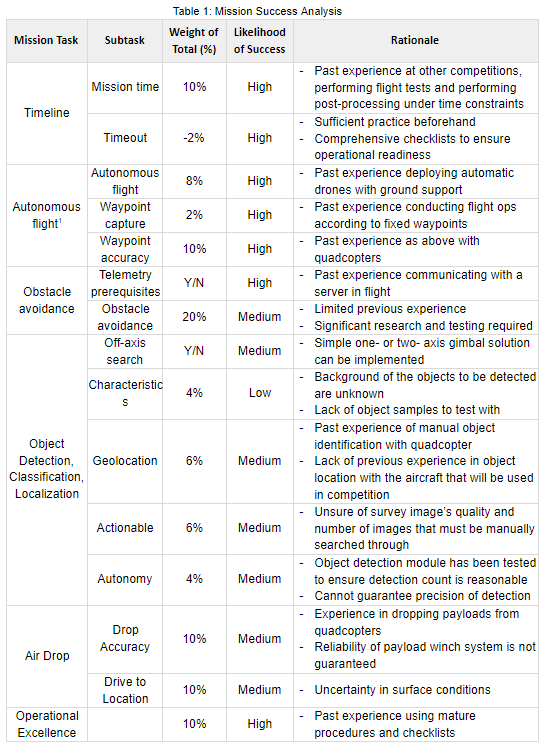
\includegraphics[height=\textheight]{table/table_1.png}
    \caption{Mission Success Analysis}
    \label{fig:msa}
\end{figure*}


\end{appendix}

% \section{Appendix}
% \clearpage

% \begin{table*}[ht]
%     \centering
%     \normalsize
%     \caption{Mission Success Analysis}
%     \label{tab:mission_success_analysis_a}

%     \begin{tabular}{p{2cm} p{2cm} p{1.5cm} p{1.5cm} p{8cm}}
%      \hline
%      Mission Task & Subtask & Weight of Total (\%) & Likelihood of Success & Rationale \\ 
%      \hline Timeline & Mission time & 10\% & High & 
%         \begin{itemize}\item Past experience at other competitions, performing flight tests and performing post-processing under time constraints \end{itemize} 
%      \\ \hline & Timeout & -2\% & High & 
%         \begin{itemize}\item Sufficient practice beforehand \item Comprehensive checklists to ensure operational readiness \end{itemize}
%      \\ \hline Autonomous flight & Autonomous flight & 8\% & High &
%         \begin{itemize}\item Past experience deploying automatic drones with ground support \end{itemize}
%      \\ \hline  & Waypoint capture & 2\% & High &
%         \begin{itemize}\item Past experience conducting flight ops according to fixed waypoints \end{itemize}
%     \\ \hline  & Waypoint accuracy & 10\% & High &
%         \begin{itemize}\item Past experience as above with quadcopters \end{itemize}
%     \\ \hline Obstacle avoidance & Telemetry prerequisites & Y/N & High &
%         \begin{itemize}\item Past experience communicating with a server in flight \end{itemize}
%     \\ \hline  & Obstacle avoidance & 20\% & High &
%         \begin{itemize}\item Limited previous experience \item Significant research and testing required
%         \end{itemize}
%   \\ \hline Object detection, classification, localization & Off-axis search & Y/N & Medium &
%         \begin{itemize}\item Simple one- or two- axis gimbal solution can be implemented 
%         \end{itemize}
%     \\ \hline & Characteristics & 4\% & Low &
%         \begin{itemize}\item Background of the objects to be detected are unknown \item Lack of object samples to test with 
%         \end{itemize}
%     \\ \hline & Geolocation & 6\% & Medium &
%         \begin{itemize}\item Past experience of manual object identification with quadcopter \item Lack of previous experience in object location with the aircraft that will be used in competition 
%         \end{itemize}
        
%     \end{tabular}


% \end{table*}

%     \clearpage
    
% \begin{table*}[ht]
%     \caption{Mission Success Analysis}
%     \label{tab:mission_success_analysis_b}
    
%     \begin{tabular}{p{2cm} p{2cm} p{1.5cm} p{1.5cm} p{8cm}}
%     \hline
%      Mission Task & Subtask & Weight of Total (\%) & Likelihood of Success & Rationale \\ 

%     \\ \hline  & Actiona
%     ble & 6\% & Medium &
%         \begin{itemize}\item Unsure of survey image’s quality and number of images that must be manually searched through  be used in competition
%         \end{itemize}
%      \\ \hline  & Autonomy & 4\% & Medium &
%         \begin{itemize}\item Object detection module has been tested to ensure detection count is reasonable \item Cannot guarantee precision of detection
%         \end{itemize}
%      \\ \hline Air drop & Drop accuracy & 10\% & Medium &
%         \begin{itemize}\item Experience dropping payloads from quadcopters \item Reliability of payload winch system is not guaranteed
%         \end{itemize}     
%     \\ \hline  & Drive to location & 10\% & Medium &
%         \begin{itemize}\item Uncertainty in surface conditions
%         \end{itemize}
%     \\ \hline Operational Excellence &  & 10\% & High &
%         \begin{itemize}\item Past experience using mature procedures and checklists \item Refined through practice
%         \end{itemize}
%      \end{tabular}
% \end{table*}

% \endinput